\documentclass[onecolumn]{article}
\usepackage{informe-lsd}
\usepackage{float}
\usepackage{pdfpages}
\usepackage{xurl}

\title{\vspace{-1.5cm}
\begin{center}
\LARGE
\textbf{Informe Técnico N.º 1 - Asistente de Investigación\\
PROYECTO PINV01-1159} \\
\Large Septiembre 2026
\vspace{0.5cm}
\end{center}
}

\author[1]{Kevin Galeano, Univ.\orcidlink{0009-0002-5536-8315}}
\affil[1]{
\small
gsmkev@gmail.com ArtICS Lab S.R.L. San Lorenzo, Paraguay.
}

\date{}

\begin{document}
\thispagestyle{firstpagestyle}
\maketitle

\vspace{-0.5cm}
\begin{abstract}
Este informe presenta un sistema de identificación automática de macroinvertebrados acuáticos que \textbf{distingue correctamente las 19 familias del conjunto de estudio}, junto con el cálculo del índice biótico BMWP que traduce esas identificaciones en una evaluación de calidad de agua. Respecto del informe anterior, el avance es de naturaleza cualitativa: el sistema pasó de tener un desempeño \emph{aparente} a tener uno \emph{verificado}.

\textbf{El aporte metodológico central del período} fue identificar y corregir un problema que afectaba al \textbf{87\,\%} del conjunto de datos y que ningún indicador de rendimiento habría revelado. El protocolo de captura fotografía cada ejemplar en series de tomas consecutivas, y esas tomas casi idénticas quedaban repartidas entre entrenamiento y evaluación, de modo que el sistema era premiado por reconocer ejemplares ya vistos. Se reconstruyó la partición agrupando por organismo, se verificó de forma independiente que ningún ejemplar aparece en dos conjuntos, y se comprobó que el procedimiento es reproducible de forma exacta. Detectar este tipo de problema es infrecuente; corregirlo y volver a medir convierte las cifras de este informe en las primeras del proyecto que un tercero puede auditar.

Sobre esa base, el sistema alcanza un \textbf{mAP@0.5:0.95 de 0.881} y un \textbf{mAP@0.5 de 0.995}, con precisión del \textbf{98.9\,\%} y exhaustividad del \textbf{97.4\,\%}. El modelo de referencia \textbf{no confunde ninguna familia con otra}: sobre las 370 fotografías de evaluación, la matriz de confusión es perfectamente diagonal. Sus únicos nueve errores son detecciones en zonas sin organismo. Dos de los tres modelos entrenados se reprodujeron \textbf{bit a bit} en una máquina distinta cuarenta y cinco días después, un grado de reproducibilidad que rara vez se documenta.

Se caracterizó además la morfometría del conjunto para entender qué condiciona la identificación. El resultado orientó el trabajo: la dificultad no proviene del tamaño de los organismos sino de su \textbf{forma}. Los taxones alargados y curvos ---larvas de díptero--- son los más difíciles de delimitar con un rectángulo, y concentran casi toda la diferencia de desempeño entre familias. Esa caracterización evitó invertir esfuerzo en técnicas de detección de objeto pequeño que no habrían servido, y define con precisión dónde queda margen de mejora.
\vspace{0.5cm}
\keywords{Detección de Objetos; YOLO; Macroinvertebrados; Bioindicadores; Calidad de Agua; Morfometría}
\end{abstract}

\section{Introducción}

El Proyecto PINV01-1159 desarrolla un sistema de monitoreo de calidad de agua superficial basado en la identificación automática de macroinvertebrados acuáticos, que funcionan como bioindicadores del estado de un curso de agua. El sistema recibe una fotografía de un ejemplar y devuelve su familia taxonómica, reemplazando una tarea que hoy requiere un especialista.

Este informe cubre el primer período del contrato (julio--septiembre de 2026) y responde a las funciones comprometidas en el Anexo I: curación del conjunto de imágenes y etiquetas, revisión de las variables de captura y de los rasgos morfológicos relevantes, pruebas de inferencia sobre imágenes no vistas, y registro de la configuración y los resultados preliminares.

El avance más significativo del período fue de naturaleza metodológica, y se describe en la Sección~\ref{sec:datos}. Auditar el conjunto de datos reveló un problema que afectaba a la mayor parte de las imágenes y que ninguna métrica de rendimiento habría delatado; corregirlo permitió establecer la \textbf{primera línea base auditable del proyecto}. Las cifras de este informe se apoyan en artefactos versionados que permiten a un tercero reproducir cada número, y el sistema quedó además operativo de extremo a extremo: identifica las familias y calcula el índice biótico que traduce esas identificaciones en una evaluación de calidad de agua.

\section{Conjunto de Datos}
\label{sec:datos}

\subsection{Composición}

El conjunto consta de \textbf{2\,403 fotografías} con \textbf{3\,032 organismos} anotados, distribuidos en \textbf{19 familias}. Son macrofotografías de ejemplar aislado sobre bandeja de laboratorio, tomadas en campañas de muestreo entre mayo y junio de 2025. La revisión de integridad de las etiquetas no encontró defectos: ninguna imagen sin anotar, ninguna coordenada fuera de rango, ninguna caja degenerada.

\begin{table}[H]
\centering
\renewcommand{\arraystretch}{1.15}
\caption{Composición del conjunto tras la corrección}
\label{tab:composicion}
\begin{tabular}{lcccc}
\hline
 & \textbf{Entrenamiento} & \textbf{Validación} & \textbf{Prueba} & \textbf{Total} \\
\hline
Fotografías          & 1\,660 & 373 & 370 & 2\,403 \\
Organismos anotados  & 2\,109 & 465 & 458 & 3\,032 \\
\textbf{Ejemplares distintos} & \textbf{473} & \textbf{81} & \textbf{87} & \textbf{641} \\
\hline
\end{tabular}
\end{table}

La distinción entre \emph{fotografías} y \emph{ejemplares distintos} es el eje de este informe: las 2\,403 fotografías corresponden a sólo 641 organismos, porque cada uno se fotografió varias veces.

\subsection{Auditoría de la partición: el hallazgo del período}

La división anterior del conjunto se hacía al azar \textbf{por fotografía}. Como cada ejemplar aparece en varias tomas casi idénticas, esas tomas quedaban repartidas entre entrenamiento y evaluación, de modo que el sistema era premiado por reconocer ejemplares ya vistos en lugar de por identificar familias.

Este tipo de problema es \textbf{particularmente difícil de detectar}, porque no produce ningún síntoma: las métricas se ven excelentes, el entrenamiento converge con normalidad y nada en el comportamiento del sistema sugiere que algo falla. Sólo aparece si se audita la estructura del conjunto de datos, que es lo que se hizo en este período.

\begin{table}[H]
\centering
\renewcommand{\arraystretch}{1.15}
\caption{Magnitud del defecto en la división original}
\label{tab:fuga}
\begin{tabular}{lc}
\hline
\textbf{Indicador} & \textbf{Valor} \\
\hline
Fotografías con tomas repartidas entre conjuntos & \textbf{2\,099 / 2\,403 (87.3\%)} \\
Imágenes de validación con una toma casi idéntica en entrenamiento & 29.2\% \\
Imágenes de prueba con una toma casi idéntica en entrenamiento & 25.6\% \\
\hline
\end{tabular}
\end{table}

La división se reconstruyó agrupando primero las fotografías por ejemplar ---dos tomas pertenecen al mismo organismo si fueron tomadas con menos de 60 segundos de diferencia o si son visualmente casi idénticas--- y repartiendo después los 641 grupos resultantes, nunca las fotografías sueltas. Un mismo ejemplar queda siempre íntegramente en un solo conjunto.

La corrección se verificó de forma independiente: ningún ejemplar aparece en dos conjuntos, las 2\,403 fotografías están asignadas, y el procedimiento es reproducible de forma exacta. La similitud residual entre conjuntos, tras la corrección, es indistinguible de la que existe naturalmente entre organismos distintos de la misma familia fotografiados con el mismo equipo.

\section{Dimensiones de los Macroinvertebrados}

Una de las funciones comprometidas fue revisar qué rasgos morfológicos condicionan la identificación automática. La caracterización que sigue permitió descartar una línea de trabajo que habría sido infructuosa y concentrar el esfuerzo donde efectivamente hay margen.

\subsection{Por qué los organismos ocupan el cuadro: una exigencia del método}

La identificación a nivel de familia no se resuelve mirando la silueta del organismo. Se resuelve mirando \textbf{caracteres diagnósticos finos}: la disposición de las sedas, la nervadura de las alas, el número y la forma de las vueltas de la concha, la segmentación de los apéndices. Esos rasgos miden fracciones de milímetro, y un especialista los examina bajo lupa. Para que un sistema automático pueda usarlos, tienen que estar \emph{resueltos en píxeles}: una fotografía general de una bandeja no los contiene, y ningún modelo puede recuperar información que la imagen no capturó.

De ahí que el protocolo sea de \textbf{macrofotografía de ejemplar aislado}: es la única forma de registrar los caracteres que la determinación taxonómica requiere. Que el organismo ocupe buena parte del cuadro no es una particularidad del conjunto, es la consecuencia necesaria de fotografiarlo con el detalle que la tarea exige.

Hay una segunda razón, menos evidente. Las familias del estudio difieren enormemente en tamaño real: un quironómido mide unos pocos milímetros, mientras que una \emph{Ampullariidae} adulta o una \emph{Hyriidae} superan varios centímetros ---dos órdenes de magnitud de diferencia---. Fotografiar todos los ejemplares a una distancia fija haría que los más pequeños quedaran reducidos a unos pocos píxeles, sin caracteres visibles, mientras los mayores saldrían del encuadre. Encuadrar cada ejemplar de modo que ocupe el cuadro \textbf{normaliza esa disparidad}: todas las familias llegan al sistema con un nivel de detalle comparable, con independencia de su tamaño físico.

\subsection{Qué implica esto para la detección}

Los sistemas de detección clasifican los objetos según el área que ocupan en la imagen. En este conjunto, \textbf{los 3\,032 organismos anotados caen en la categoría de objeto grande}, sin una sola excepción. El ejemplar más pequeño del conjunto ocupa tres veces el umbral de esa categoría, y el organismo típico ocupa el \textbf{52.6\% del cuadro}.

\begin{figure*}[!t]
  \centering
  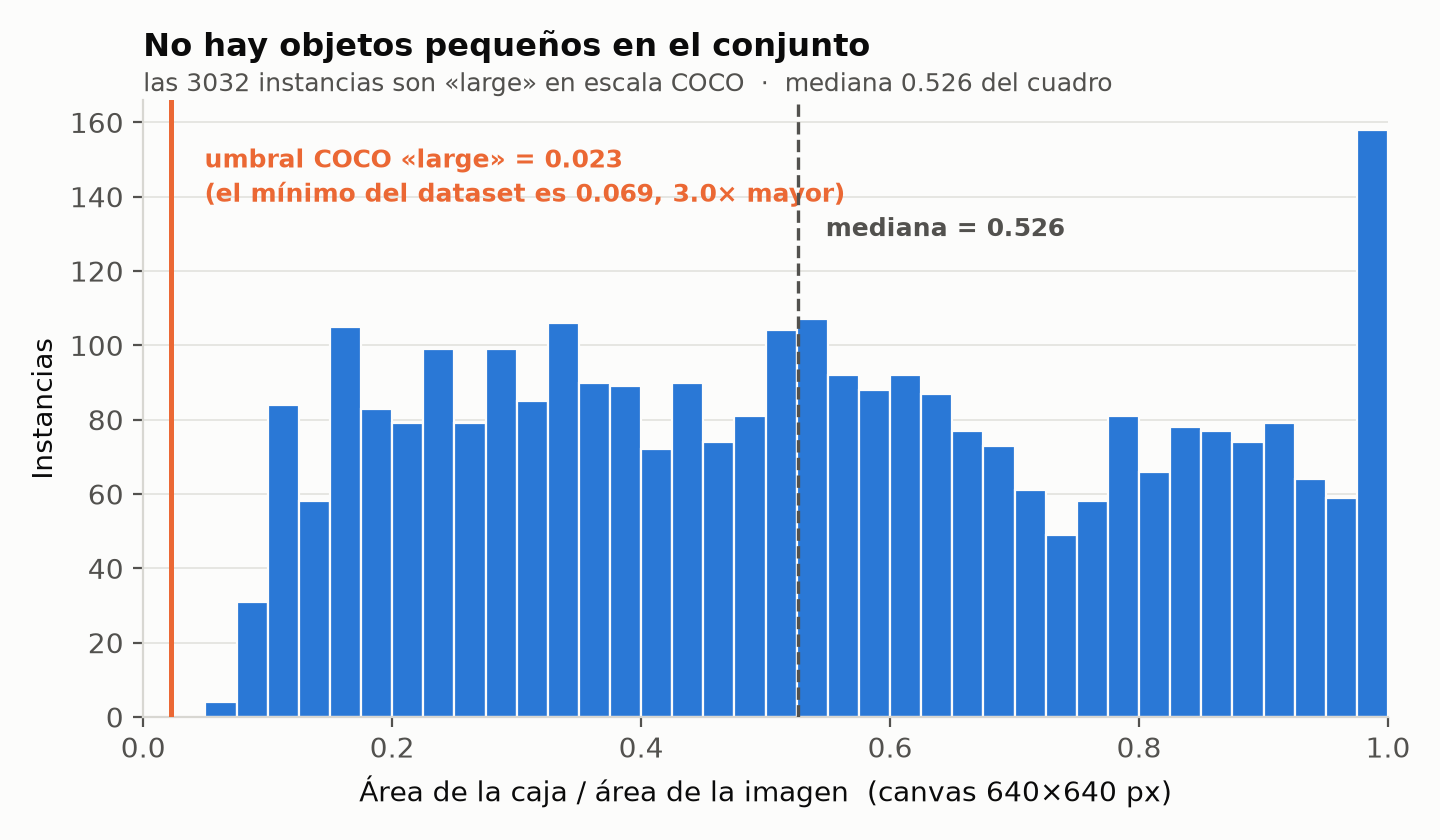
\includegraphics[width=0.8\linewidth]{imagenes/distribucion_tamanos_bbox.png}
  \caption{Superficie que ocupa cada organismo dentro de la fotografía. No hay ejemplares en el régimen de objeto pequeño, donde las técnicas habituales de detección fina serían necesarias.}
  \label{fig:tamanos}
\end{figure*}

En términos prácticos esto es una ventaja: el sistema no necesita resolver el problema de la detección de objetos pequeños, que es donde los detectores modernos concentran sus dificultades. La caracterización permitió descartar desde el principio las técnicas asociadas a ese régimen ---aumento de resolución, procesamiento por mosaicos, cabezas de detección a escalas finas---, que habrían consumido esfuerzo sin retorno.

\subsection{La forma sí lo es}

Lo que sí predice la dificultad es la \textbf{elongación}: cuán alargado es el organismo. La relación es fuerte ---explica alrededor del \textbf{70\%} de la diferencia de desempeño entre familias--- mientras que el tamaño no muestra relación significativa. Con sólo 19 familias, ese 70\% tiene un intervalo de confianza ancho (entre 38\% y 88\%): lo que el dato sostiene con firmeza es el \emph{orden}, no la magnitud exacta.

\begin{figure*}[!t]
  \centering
  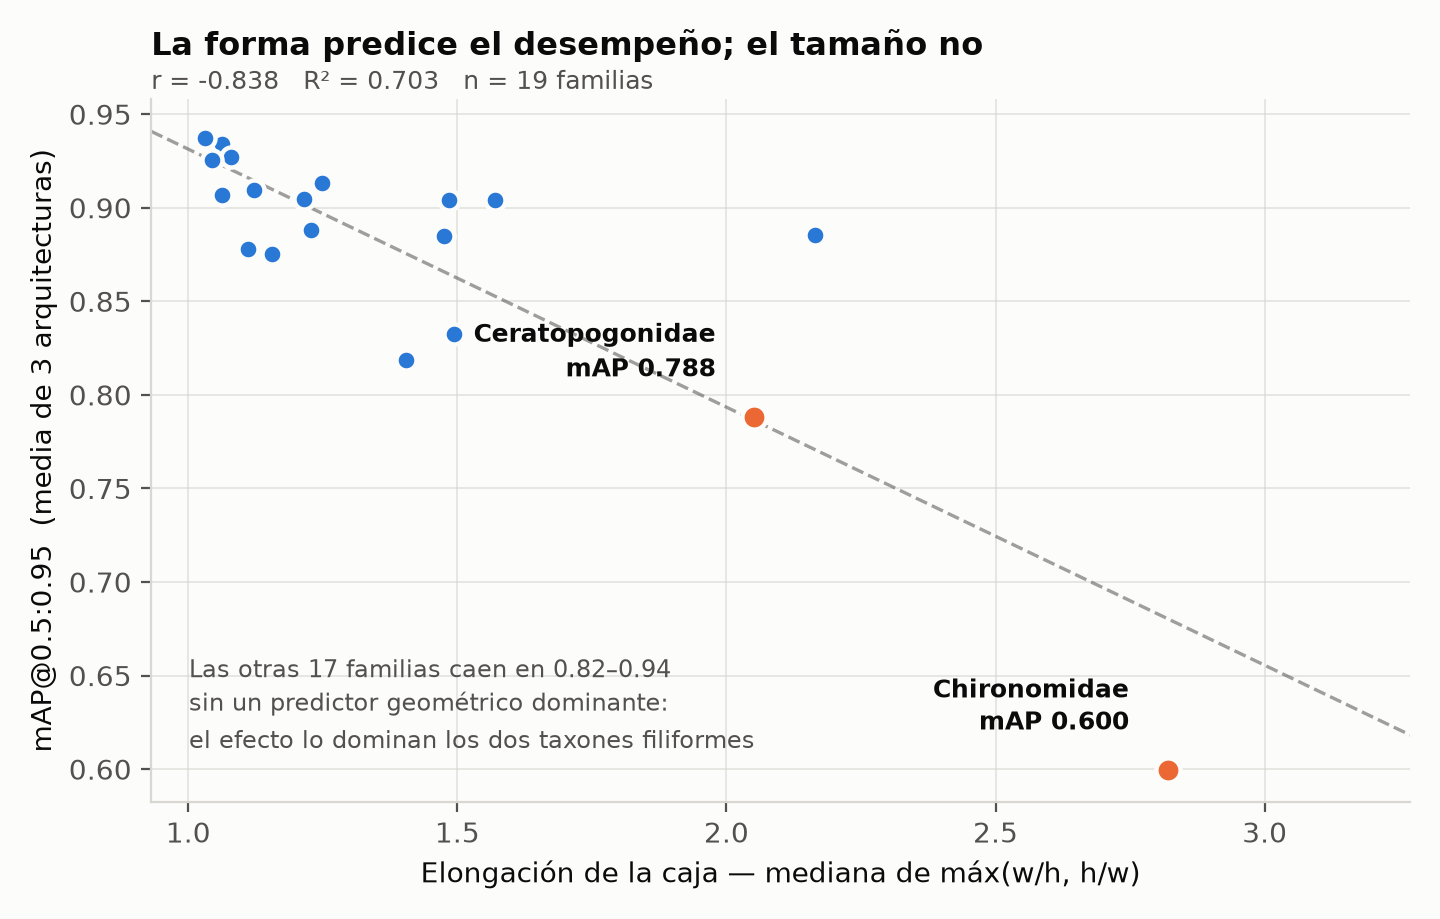
\includegraphics[width=0.8\linewidth]{imagenes/elongacion_vs_map.png}
  \caption{Desempeño por familia frente a la elongación del organismo. \emph{Chironomidae} y \emph{Ceratopogonidae} concentran la dificultad; las 17 familias restantes rinden entre 0.82 y 0.94.}
  \label{fig:elongacion}
\end{figure*}

El motivo es geométrico. El sistema delimita cada organismo con un rectángulo alineado a los bordes de la imagen. Para un ejemplar compacto, ese rectángulo lo contiene con precisión. Para una larva filiforme y curva, el rectángulo contiene mayoritariamente fondo, y su contorno exacto depende de cómo haya quedado el organismo sobre la bandeja: dos especialistas trazarían rectángulos distintos.

\begin{figure*}[!t]
  \centering
  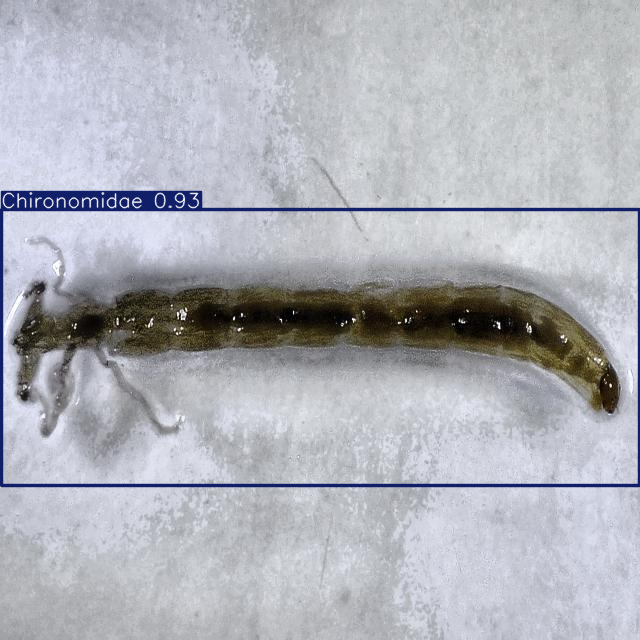
\includegraphics[width=0.55\linewidth]{imagenes/ejemplo_dificil.png}
  \caption{Identificación correcta de \emph{Chironomidae}, la familia de menor desempeño. La familia se reconoce sin ambigüedad; lo que resulta impreciso es el rectángulo que la delimita, que encierra sobre todo sustrato.}
  \label{fig:dificil}
\end{figure*}

\paragraph{Enfoque adoptado.} De esta caracterización se derivaron tres decisiones:

\begin{enumerate}
  \item \textbf{No invertir en técnicas de objeto pequeño.} Habrían consumido esfuerzo sin retorno, porque el problema que resuelven no existe en este conjunto.
  \item \textbf{Evaluar con una métrica exigente en la delimitación} (mAP@0.5:0.95), porque las métricas más permisivas se saturan en este tipo de imágenes y dejan de distinguir entre un sistema bueno y uno mediocre.
  \item \textbf{Interpretar la penalización de los taxones alargados como un límite del método de anotación}, no como una falla del sistema. Para el uso ecológico lo relevante es acertar la familia, no el contorno exacto del rectángulo.
\end{enumerate}

\paragraph{Alcance de la afirmación.} El efecto está dominado por las dos familias de peor desempeño, \emph{Chironomidae} y \emph{Ceratopogonidae}: excluyéndolas, la relación entre forma y desempeño cae de $-0.84$ a $-0.43$ y deja de ser clara. Lo que sostienen los datos es que \emph{esas dos larvas filiformes son marcadamente más difíciles que el resto}, no que exista una regla general que vincule forma y desempeño en todo el conjunto.

\section{Resultados}

Se entrenaron y compararon tres arquitecturas sobre la división corregida. Todas usan fotografías de $640\times640$ px y una estrategia de aumentación agresiva, destinada a evitar que el sistema se apoye en el fondo de la bandeja en lugar del organismo.

\paragraph{Sobre la tasa de aprendizaje.} No se fijó a mano: se delegó en el mecanismo automático de la biblioteca, que para un conjunto de este tamaño selecciona el optimizador AdamW con una tasa de $4.35\times10^{-4}$. El valor $0.01$ que figura en los archivos de configuración corresponde a otro optimizador y \textbf{el mecanismo automático lo descarta explícitamente}; no fue el valor efectivo. La tasa real quedó verificada contra el registro que cada modelo guarda de su propio entrenamiento.

Tampoco se hizo un barrido de ese parámetro, por dos razones. Las curvas de entrenamiento no muestran que la tasa sea el límite: los tres modelos alcanzan el 98\,\% de su desempeño máximo hacia la época 113 y luego se mantienen planos, mientras el error sobre los datos de entrenamiento sigue bajando y el de validación repunta. Esa combinación indica que el techo lo pone la \textbf{cantidad de datos}, no el ritmo de aprendizaje. Y aunque lo pusiera, la incertidumbre de este conjunto ---con 87 ejemplares independientes--- supera la diferencia observada entre las tres arquitecturas: un ajuste de este tipo produciría un efecto que no se podría medir. La exploración de hiperparámetros se pospone a cuando el conjunto de evaluación sea mayor.

\paragraph{El calendario de entrenamiento: un ajuste que se probó y no sirvió.} El descenso programado de la tasa de aprendizaje y la fase final sin aumentación se calendarizan contra el presupuesto \emph{solicitado} de 200 épocas, pero la parada temprana interrumpía las corridas antes, de modo que esa fase final nunca llegaba a ejecutarse en dos de los tres modelos. Se corrigió y se repitió el entrenamiento completo.

\textbf{El resultado fue el contrario del esperado.} La fase sin aumentación \emph{degrada} el desempeño en los tres modelos ---entre 0.2 y 1.8 puntos respecto de la meseta previa, sin recuperarse antes del final--- y el mecanismo quedó medido: en esas últimas quince épocas el error sobre los datos de entrenamiento cae un 43\,\%, mientras el de validación sube. Es sobreajuste. Con 1 660 fotografías, un solo organismo por imagen y el efecto del contexto fotográfico descrito en la Sección~\ref{sec:futuro}, la aumentación no es un accesorio: es la principal fuente de regularización del entrenamiento, y retirarla perjudica.

Dos de los tres modelos ---incluido el de referencia--- resultaron \textbf{idénticos} a los de la primera corrida: no sólo el mismo desempeño, sino los mismos pesos, sin una sola diferencia en ninguno de sus más de setecientos tensores, reproducidos cuarenta y cinco días después en otra computadora. Es un resultado de reproducibilidad que vale por sí mismo: el procedimiento descrito acá regenera exactamente los modelos que reporta. El tercer modelo varió dentro del ruido. Las cifras, por lo tanto, no eran una cota inferior: eran ya el techo de esta configuración.

\paragraph{Lo que este ajuste sí costó.} Desactivar la parada temprana amplía en un 28\,\% el número de épocas entre las que se elige el mejor modelo, y esa elección se hace sobre el conjunto de validación, que tiene 81 ejemplares. Cuantos más candidatos, mayor la probabilidad de que el elegido lo sea por azar favorable y no por mérito. Es lo que le ocurrió al tercer modelo: mejoró una décima de punto en validación y empeoró otra en prueba. Queda declarado como límite del procedimiento de selección, no como resultado.

\begin{table}[H]
\centering
\renewcommand{\arraystretch}{1.15}
\caption{Desempeño sobre el conjunto de prueba: 370 fotografías, 458 organismos, 87 ejemplares no usados en el entrenamiento. Protocolo estándar de evaluación ($\tau=0.001$, IoU$=0.7$); la precisión y la exhaustividad en el punto de operación del sistema ($\tau=0.30$) figuran más abajo.}
\label{tab:metricas}
\begin{tabular}{lccccc}
\hline
\textbf{Modelo} & \textbf{mAP@0.5} & \textbf{mAP@0.5:0.95} & \textbf{Precisión} & \textbf{Exhaustividad} & \textbf{F1} \\
\hline
YOLO11s & 0.993 & 0.864 & 98.8\% & 96.0\% & 0.974 \\
YOLO12s & 0.995 & 0.879 & 99.1\% & 99.8\% & 0.994 \\
\textbf{YOLO26s} & 0.995 & \textbf{0.881} & 98.9\% & 97.4\% & 0.982 \\
\hline
\end{tabular}
\end{table}

Las tres arquitecturas rinden prácticamente igual. Para dimensionar la incertidumbre, los intervalos se calculan remuestreando los \textbf{87 ejemplares distintos}, no las 370 fotografías: varias tomas del mismo organismo no son observaciones independientes, y tratarlas como tales estrecha el intervalo en un factor cercano a 1.5. En el punto de operación ($\tau=0.30$), el modelo de referencia da \textbf{precisión 98.9\,\%}, \textbf{exhaustividad 97.9\,\%} y \textbf{F1 0.984} sobre validación. Los intervalos de confianza son más anchos que las diferencias entre arquitecturas, de modo que \textbf{el informe no declara una arquitectura ganadora}. YOLO26s se adopta como modelo de referencia por tener el mejor valor puntual.

El umbral de confianza con el que opera el sistema (0.30) se fijó mediante un barrido sobre el conjunto de validación. El valor óptimo resultó 0.25, pero la diferencia con 0.30 es de una milésima de F1 y 0.30 comete menos falsos positivos. Se conservó por esa razón: en un sistema de bioindicación, un falso positivo introduce una familia inexistente en el recuento y distorsiona el índice de calidad de agua, mientras que un falso negativo sólo lo empobrece.

\subsection{Desempeño por familia}

\begin{table}[H]
\centering
\renewcommand{\arraystretch}{1.1}
\small
\caption{Desempeño por familia (mAP@0.5:0.95, promedio de las tres arquitecturas), ordenado de menor a mayor}
\label{tab:familias}
\begin{tabular}{lcc|lcc}
\hline
\textbf{Familia} & \textbf{mAP} & \textbf{Elong.} & \textbf{Familia} & \textbf{mAP} & \textbf{Elong.} \\
\hline
Chironomidae     & \textbf{0.600} & \textbf{2.82} & Hydrophilidae  & 0.904 & 1.48 \\
Ceratopogonidae  & \textbf{0.788} & \textbf{2.05} & Hyriidae       & 0.905 & 1.22 \\
Ancylidae        & 0.819 & 1.41 & Gerridae       & 0.907 & 1.06 \\
Psychodidae      & 0.833 & 1.49 & Notonectidae   & 0.910 & 1.12 \\
Noteridae        & 0.875 & 1.16 & Planorbidae    & 0.913 & 1.25 \\
Physidae         & 0.878 & 1.11 & Miridae        & 0.925 & 1.04 \\
Glossiphoniidae  & 0.885 & 1.47 & Dytiscidae     & 0.927 & 1.08 \\
Hirudinidae      & 0.885 & 2.17 & Belostomatidae & 0.934 & 1.06 \\
Ampullariidae    & 0.888 & 1.23 & Libellulidae   & 0.937 & 1.03 \\
Coenagrionidae   & 0.904 & 1.57 & & & \\
\hline
\end{tabular}
\end{table}

El orden es estable entre las tres arquitecturas: las mismas familias son las más difíciles en todos los casos, lo que confirma que la dificultad es una propiedad del taxón y no de una corrida de entrenamiento particular. Con entre 2 y 7 ejemplares por familia en el conjunto de prueba, estas cifras deben leerse como indicativas.

\begin{figure*}[!t]
  \centering
  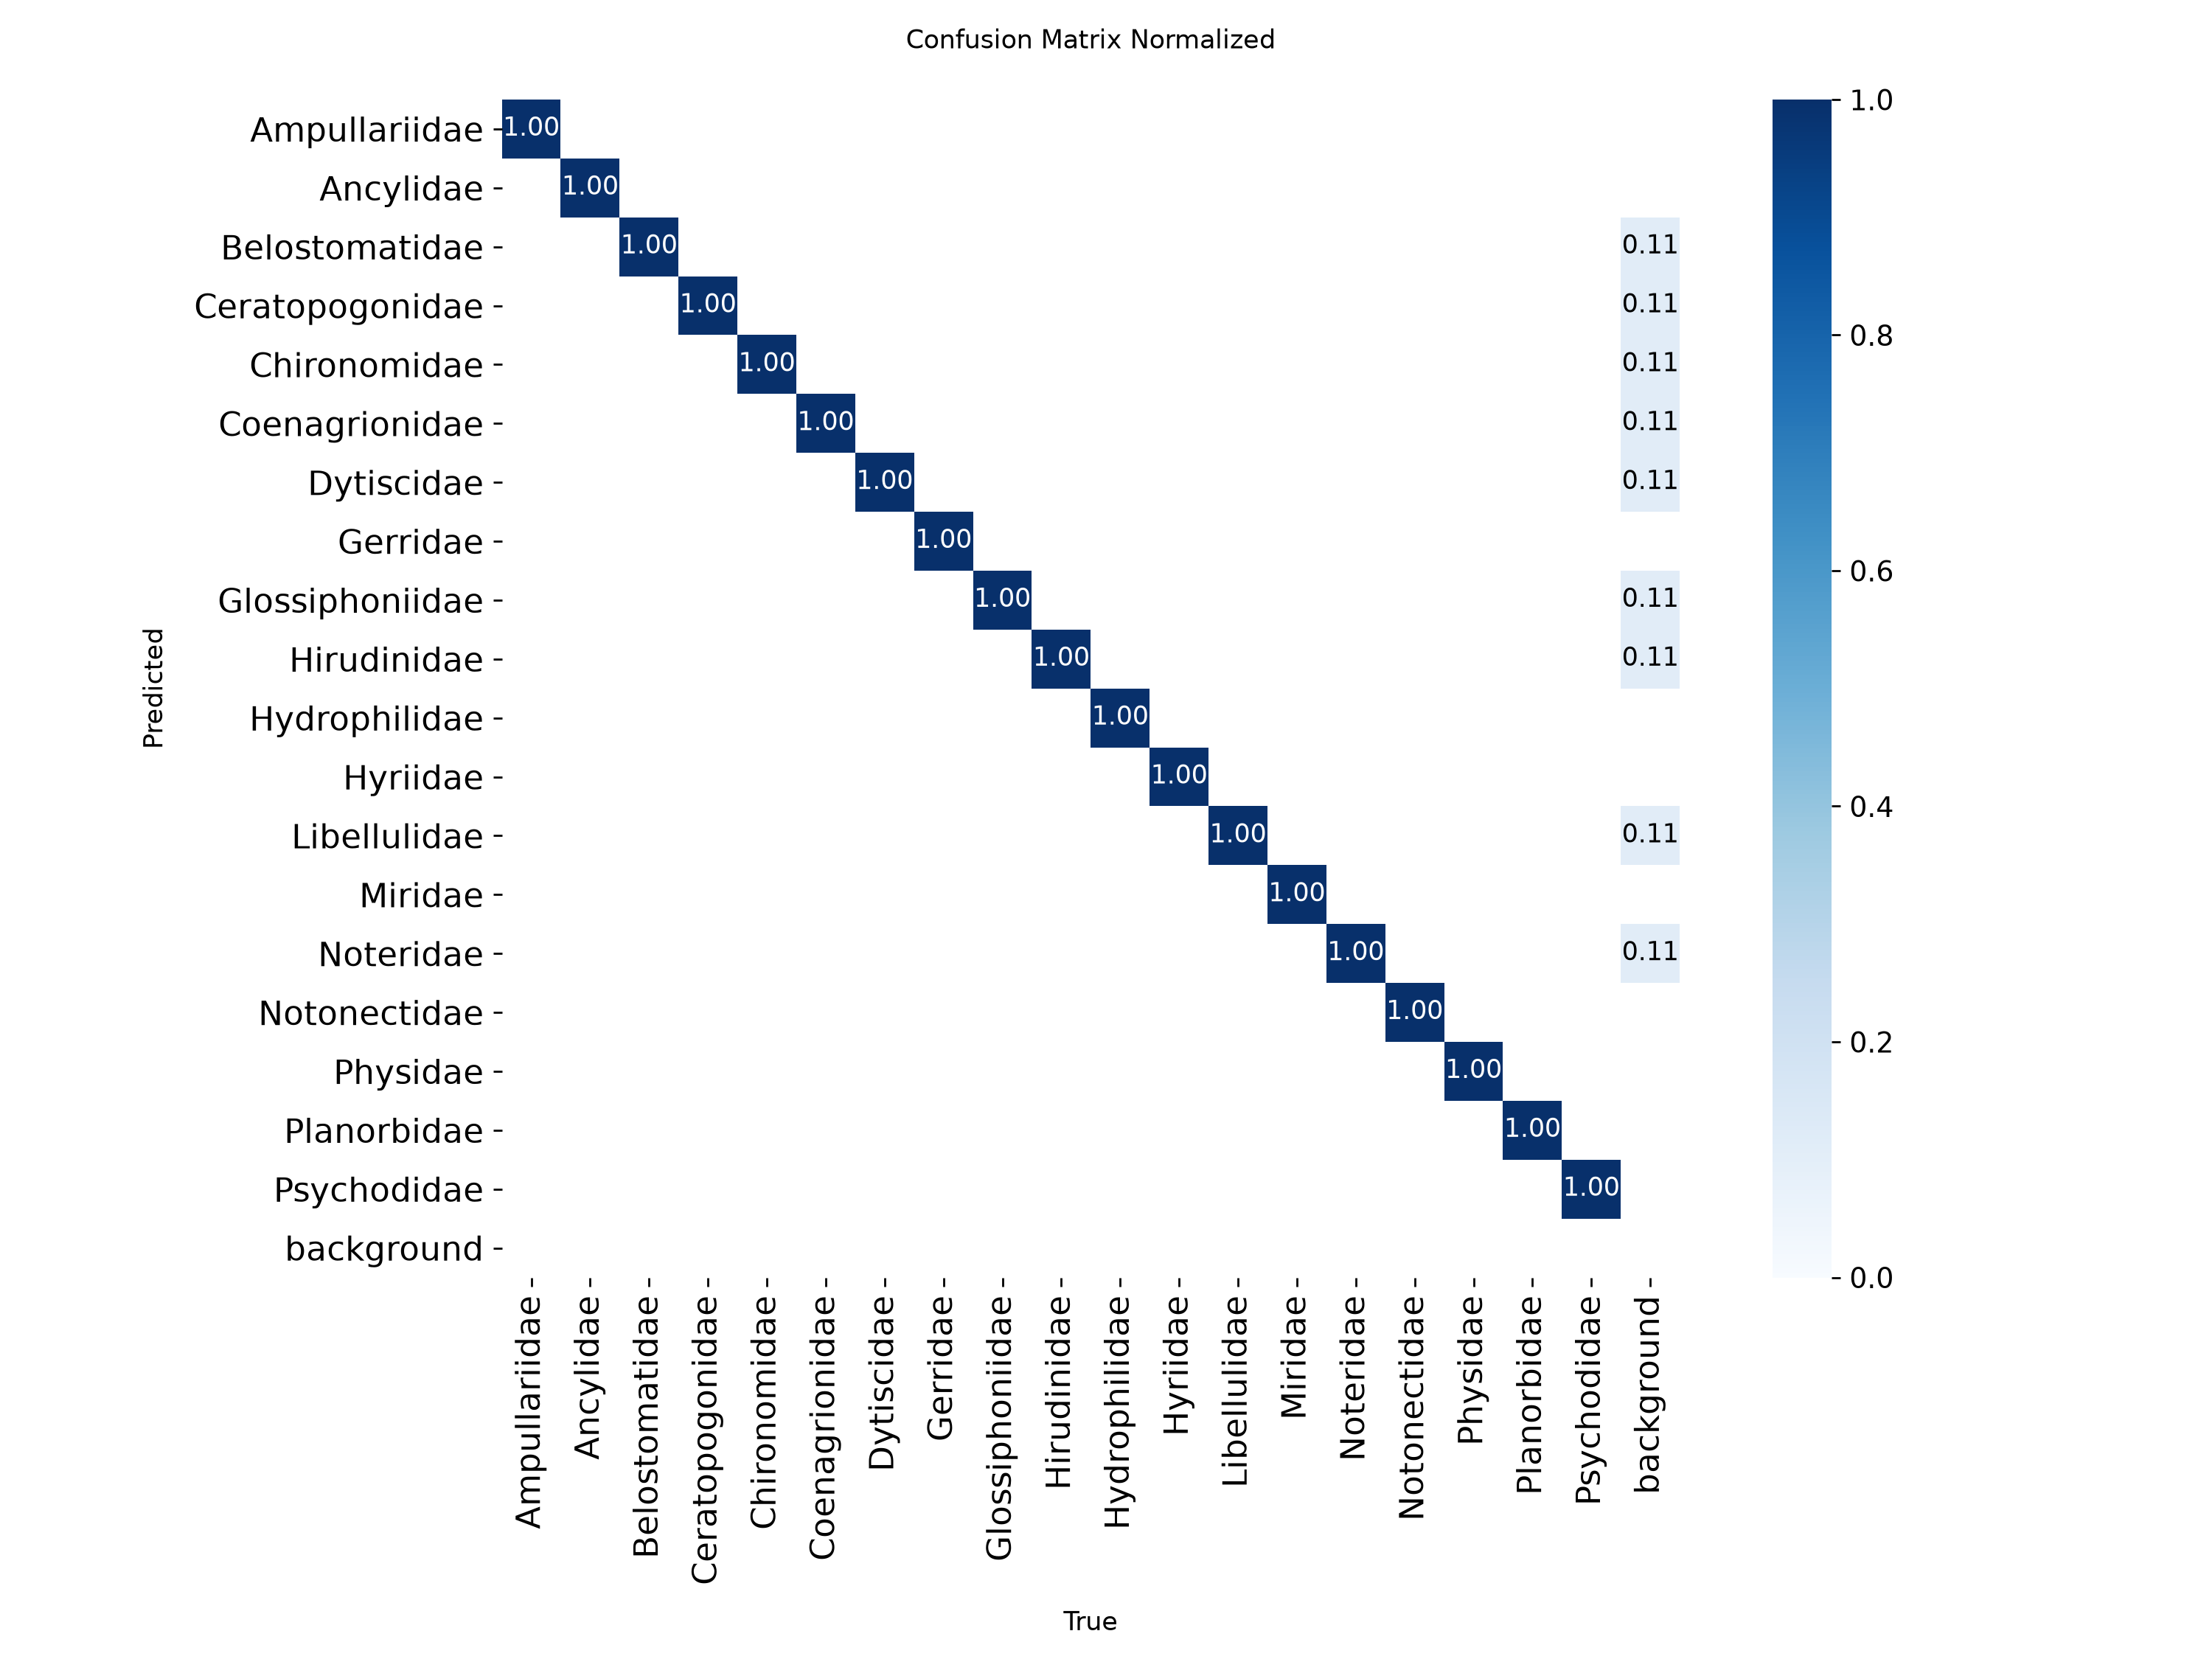
\includegraphics[width=0.8\linewidth]{imagenes/confusion_matrix_normalized.png}
  \caption{Matriz de confusión sobre el conjunto de prueba. \textbf{El modelo de referencia no confunde ninguna familia con otra: la diagonal está limpia.} Los nueve errores del modelo son detecciones donde no había organismo, repartidas una por familia. Es el tipo de error que la campaña complementaria permitirá cuantificar: el conjunto no contiene todavía ninguna fotografía sin organismo, de modo que la tasa real de detecciones espurias no está medida y estos nueve casos son sólo los que aparecen en imágenes que sí contienen un ejemplar.}
  \label{fig:confusion}
\end{figure*}

\begin{figure*}[!t]
  \centering
  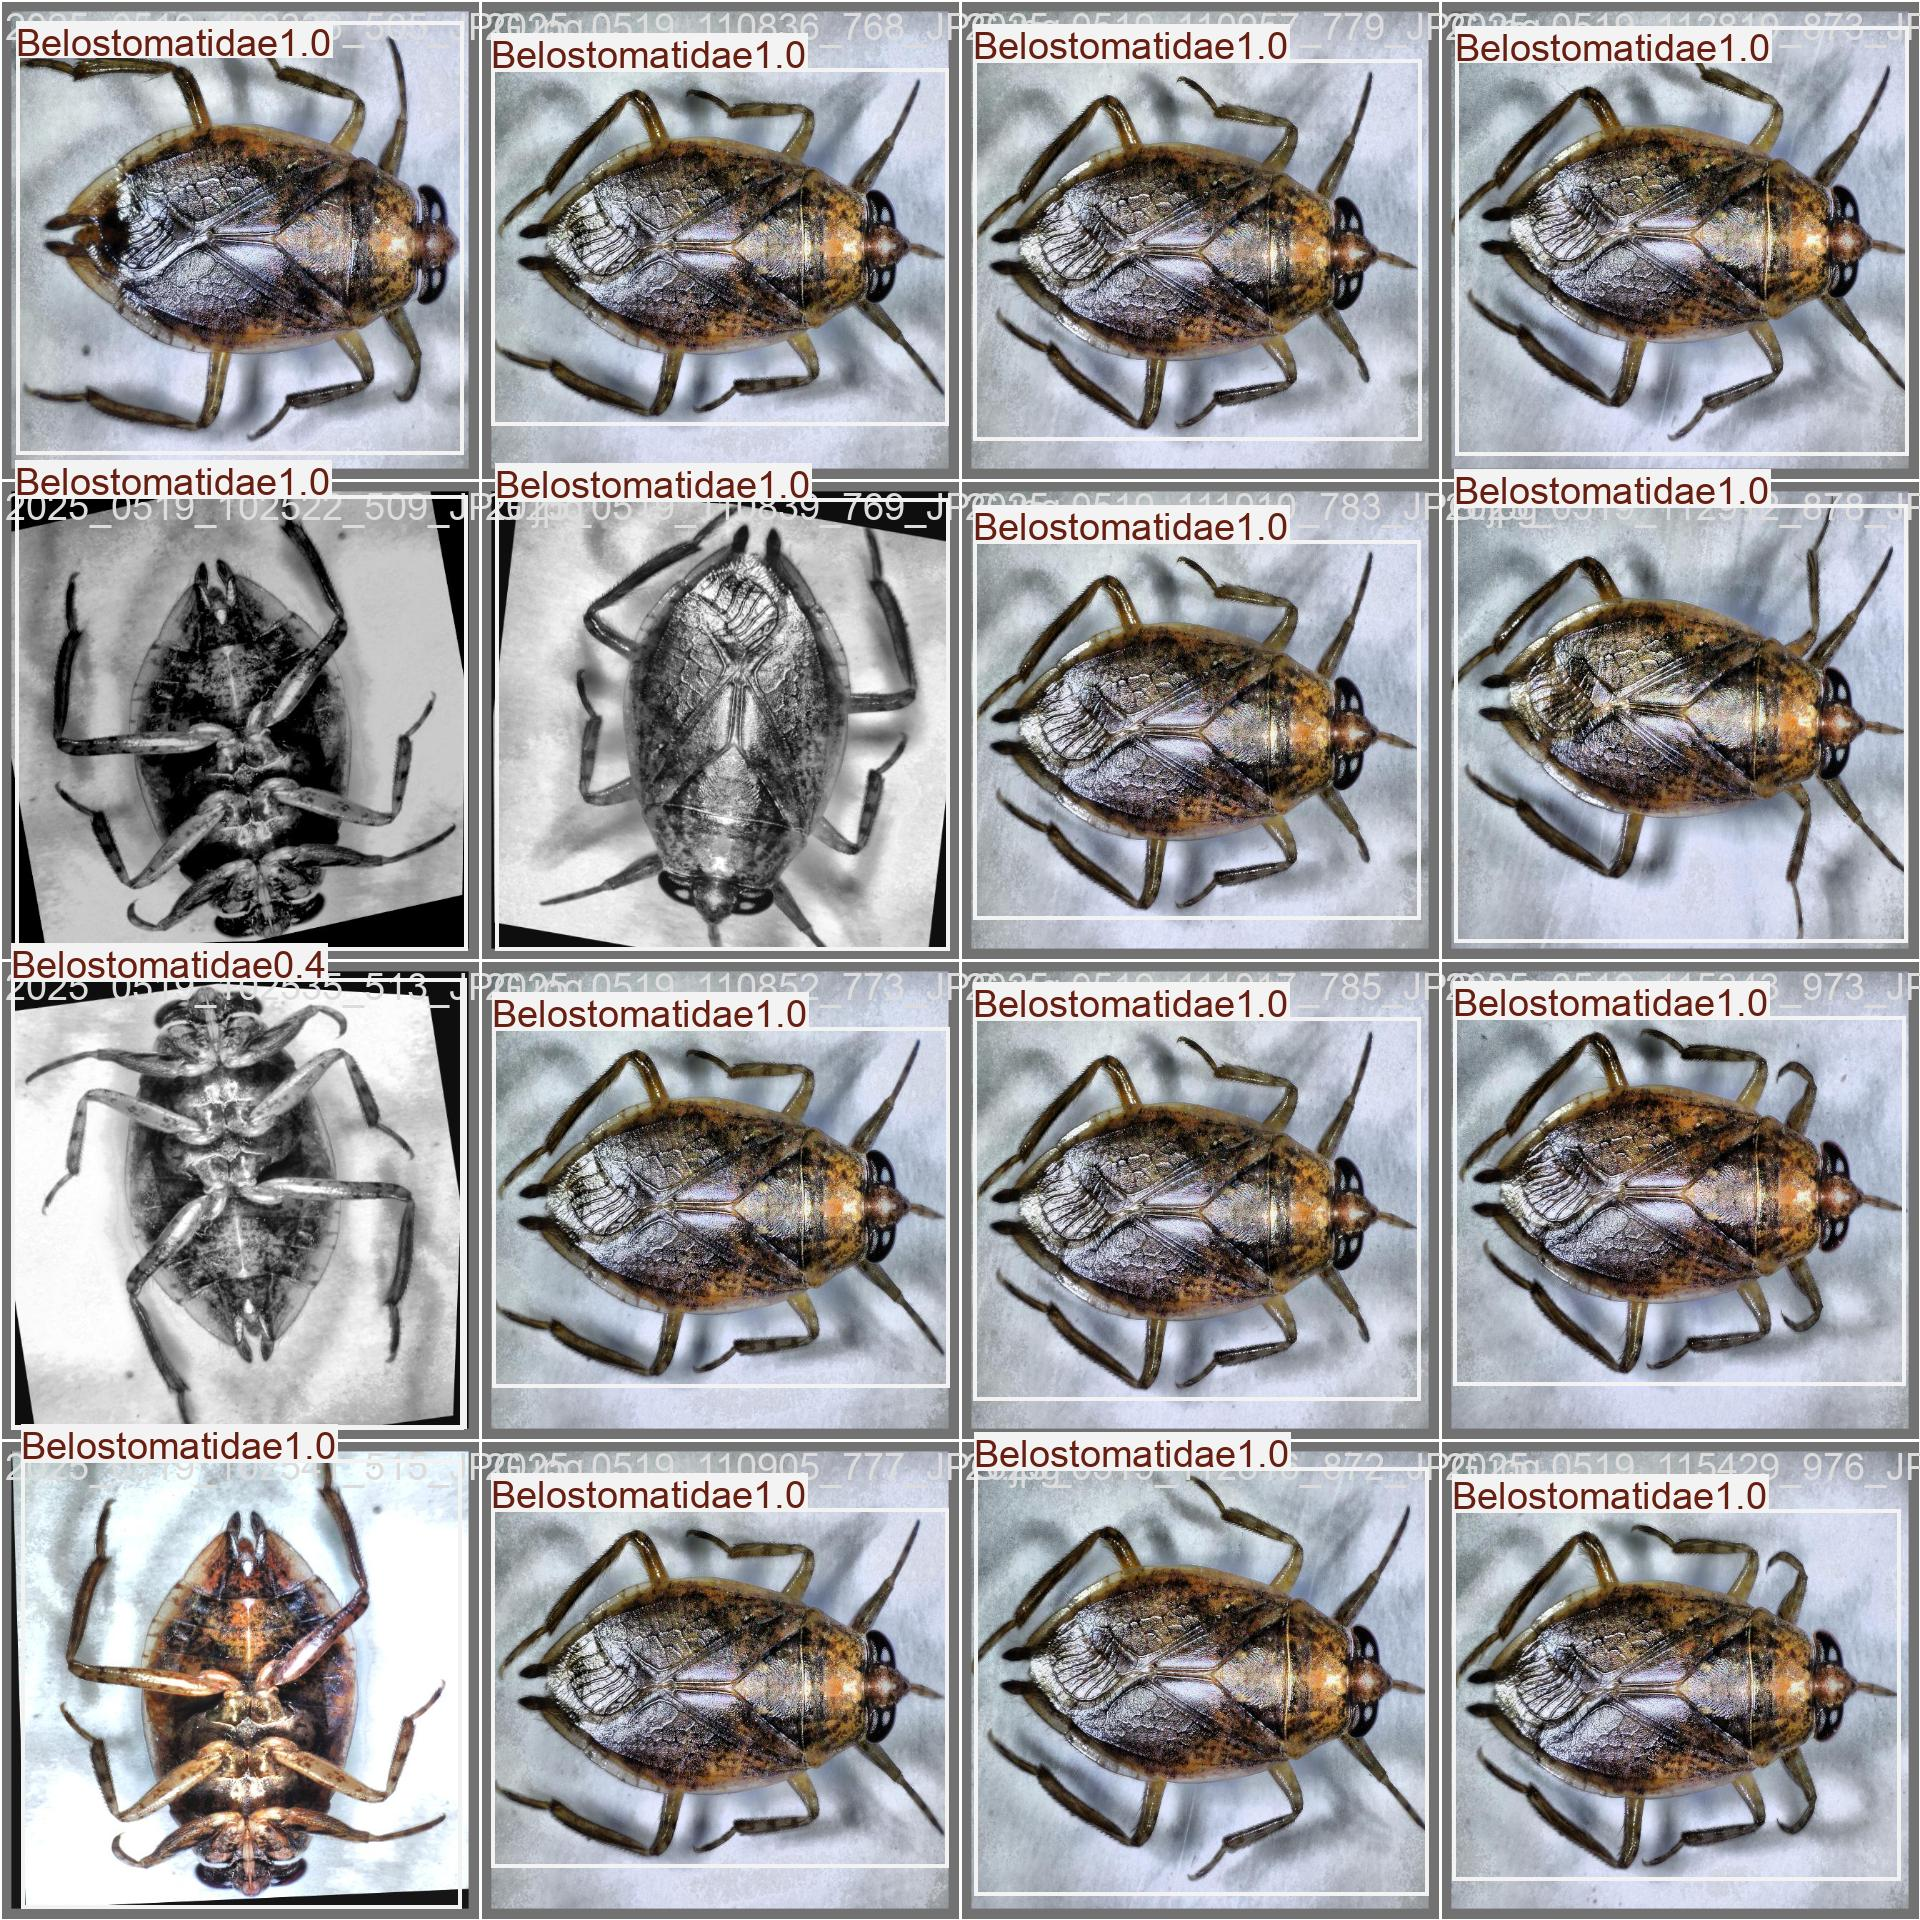
\includegraphics[width=0.92\linewidth]{imagenes/pipeline_validacion.jpg}
  \caption{Salida del pipeline de evaluación sobre un lote del conjunto de prueba, generada automáticamente durante la validación. Cada recuadro muestra la familia identificada y su confianza.}
  \label{fig:pipeline}
\end{figure*}

\begin{figure*}[!t]
  \centering
  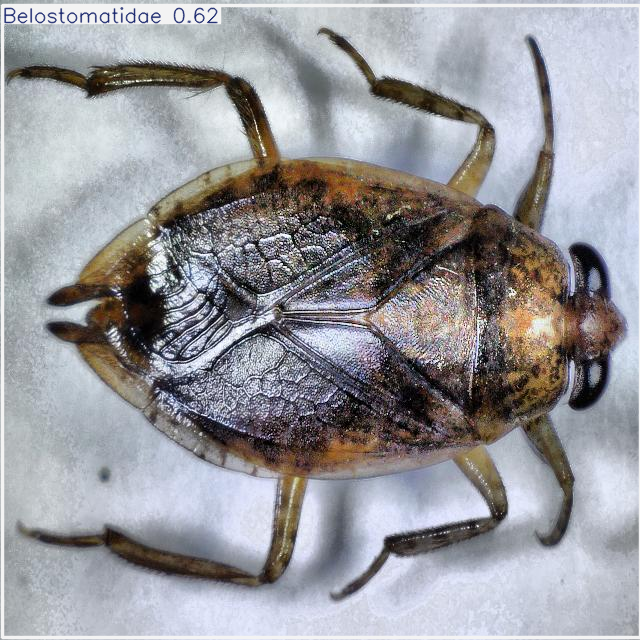
\includegraphics[width=0.55\linewidth]{imagenes/ejemplo_simple.png}
  \caption{Identificación de un ejemplar aislado de \emph{Belostomatidae}, el régimen de captura para el que el sistema está validado.}
  \label{fig:simple}
\end{figure*}

\begin{figure*}[!t]
  \centering
  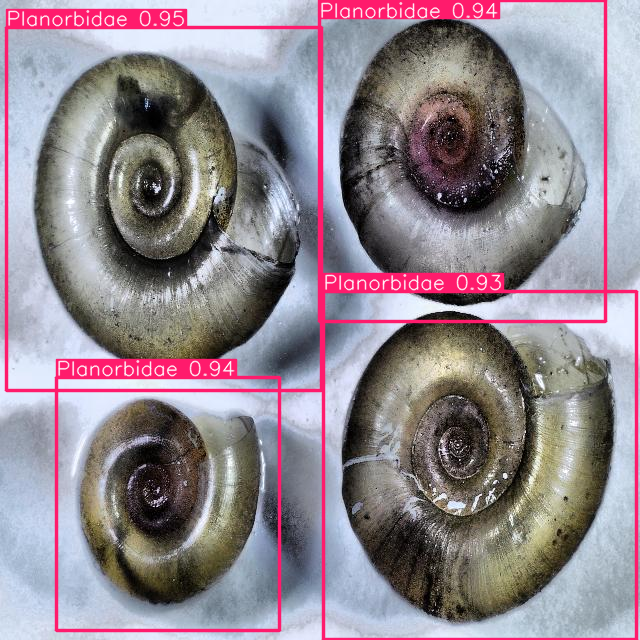
\includegraphics[width=0.55\linewidth]{imagenes/ejemplo_multiple.png}
  \caption{Identificación simultánea de cuatro ejemplares de \emph{Planorbidae} en una misma fotografía, todos recuperados con alta confianza. Es el caso de mayor número de organismos del conjunto de prueba.}
  \label{fig:multiple}
\end{figure*}

\subsection{Qué se ganó respecto del informe anterior}

El informe de avance previo reportaba 99.9\,\% de precisión y 100\,\% de exhaustividad. Esas cifras se obtuvieron sobre la partición que este período identificó como defectuosa, de modo que las de la Tabla~\ref{tab:metricas} las reemplazan. La diferencia entre ambos informes no está en el desempeño del sistema, sino en \textbf{qué tan bien se lo conoce}.

Conviene explicar por qué las cifras se mueven tan poco. En fotografías donde un solo organismo ocupa la mitad del cuadro, la precisión y la exhaustividad se saturan cerca del 100\,\% con el defecto y sin él: no eran capaces de revelarlo, y por eso el problema pasó inadvertido. El avance de este período consistió precisamente en \textbf{dejar de depender de métricas que no discriminan}. El mAP@0.5:0.95 ---que el informe anterior no reportaba--- sí distingue la calidad de la delimitación, se ubica en 0.881, y señala con precisión dónde queda margen.

En concreto, este informe suma sobre el anterior: una partición verificada y reproducible, una métrica capaz de discriminar, la comparación de tres arquitecturas bajo idéntico protocolo, la caracterización morfométrica que orientó las decisiones de diseño, el índice biótico operativo, y un conjunto de artefactos versionados que permiten auditar cada cifra.

\section{Alcance de Validez y Trabajo Futuro}
\label{sec:futuro}

\subsection{Para qué está validado el sistema}

Los resultados de este informe corresponden a \textbf{macrofotografía de ejemplar aislado sobre bandeja de laboratorio}, que es el protocolo descrito en la Sección~\ref{sec:datos} y el que la determinación taxonómica requiere. Dentro de ese régimen el sistema está medido y es reproducible. Fuera de él ---bandejas con varios organismos de familias distintas, o fotografía en el terreno--- todavía no hay medición, y ampliarla es el primer punto de la agenda que sigue.

Conviene además explicitar el tamaño de la evidencia: el conjunto de evaluación contiene 87 ejemplares independientes, entre 2 y 7 por familia. Las cifras globales son sólidas; las de familias individuales deben leerse como indicativas.

\subsection{Trabajo futuro}

La agenda del período final surge de mediciones hechas en éste, no de conjeturas. Ordenada por impacto:

\begin{enumerate}
  \item \textbf{Campaña de captura complementaria.} Es la acción de mayor retorno, porque habilita por sí sola tres de los avances siguientes, y la única que requiere planificación anticipada. Comprende tres componentes:
  \begin{itemize}
    \item \textbf{Al menos tres jornadas por familia}, con distinto fondo, bandeja e iluminación. Hoy doce de las diecinueve familias provienen de una sola jornada, y eso hace que el contexto fotográfico sea parcialmente predictivo de la clase. Está \textbf{cuantificado}: un clasificador trivial sobre miniaturas de $32\times32$ píxeles en gris ---donde el organismo es apenas un borrón--- acierta la familia el \textbf{39.5\,\%} de las veces frente al 5.3\,\% esperable por azar, y una ablación que tapa al organismo muestra que el sistema mantiene la predicción correcta en torno al 16\,\% de los casos. Diversificar las sesiones elimina esa vía y permitirá reservar una jornada completa por familia como evaluación independiente.
    \item \textbf{Fotografías de bandeja sin organismo}, que permitirán medir por primera vez la tasa de detecciones espurias ---hoy los nueve únicos errores del modelo son exactamente de ese tipo.
    \item \textbf{Fotografías de bandeja de muestreo con varios ejemplares}, que es el régimen operativo de destino.
  \end{itemize}
  \item \textbf{Ampliación del número de ejemplares por familia}, que estrechará los intervalos de confianza y permitirá afirmar diferencias que hoy quedan dentro del ruido.
  \item \textbf{Validación del sistema contra identificación experta} sobre las imágenes nuevas, familia por familia.
  \item \textbf{Validación taxonómica documentada} de las diecinueve familias, y cierre del índice biótico. El cálculo del BMWP ya está implementado y operativo ---presencia/ausencia, agregado por sitio de muestreo, con el índice complementario ASPT---, y discrimina correctamente entre sitios de distinta calidad. Resta la revisión de un especialista, en particular para \emph{Hyriidae} y \emph{Miridae}, que no figuran en las tablas de referencia y cuyo puntaje el sistema declara hoy como provisional en cada resultado.
  \item \textbf{Documentación técnica final} del sistema y del flujo completo desde la fotografía hasta el índice biológico.
\end{enumerate}

\paragraph{Una línea ya explorada, y su resultado.} Antes de orientar el esfuerzo hacia la captura se probaron tres técnicas para que el sistema dejara de apoyarse en el contexto fotográfico, sin modificar el conjunto de datos: aumentación agresiva de color y geometría, recorte y pegado del organismo sobre fondos de otras sesiones en dos volúmenes distintos, y una penalización en la función de pérdida que castiga la atención fuera del organismo. \textbf{Ocho corridas independientes sobre tres arquitecturas dejaron el resultado entre 15.7\,\% y 16.6\,\%}, un rango demasiado estrecho para atribuirle efecto a ninguna intervención. La conclusión es útil y ahorra trabajo: mientras la señal esté presente en los píxeles de entrada, el entrenamiento tiene incentivo para usarla, y ninguna técnica aplicada \emph{sobre el modelo} la elimina. Por eso el período final apunta a los datos y no al ajuste del entrenamiento.

\paragraph{Estado al cierre del período.} El proyecto cuenta con un conjunto curado y verificado, una partición metodológicamente correcta y reproducible, tres arquitecturas entrenadas y evaluadas bajo idéntico protocolo, una caracterización morfométrica que orientó las decisiones de diseño, y el índice biótico operativo de extremo a extremo. Con la campaña complementaria, el proyecto puede cerrar en diciembre con un sistema evaluado en las condiciones en que va a usarse.

\section{Medios de Verificación}

\begin{itemize}
    \item \textbf{Código y documentación del sistema}: \url{https://github.com/pinv01-1159/yolo-macro-detect}
    \item \textbf{Conjunto de datos con la división corregida}: \url{https://app.roboflow.com/pinv011159/macroinvertebrados-split-limpio-kuhq3}
    \item \textbf{Modelos entrenados}, con registro de su configuración, entorno de ejecución y versión del código: carpeta \texttt{checkpoints} del repositorio.
    \item \textbf{Auditoría técnica independiente} del conjunto de datos, la división y las métricas, con el detalle de los procedimientos de verificación: \path{reports/paper/auditoria.md}.
    \item \textbf{Registro de variables} de captura, morfométricas, de entrenamiento y de inferencia, con la procedencia de cada valor: \path{reports/paper/variables_modelo.md}.
    \item \textbf{Análisis de la fuga de datos y su corrección}, con la medición del defecto original y la verificación de la división reconstruida: \path{docs/leakage_analysis.md}.
    \item \textbf{Resultados de evaluación} por familia y matrices de confusión, en formato tabular: carpeta \texttt{reports/paper} del repositorio.
    \item \textbf{Procedencia de cada artefacto} ---huella SHA-256, comando que lo regenera y \emph{commit} del código---: \path{reports/paper/provenance.json}.
\end{itemize}

Todas las cifras de este informe provienen de esos artefactos y pueden regenerarse a partir del repositorio.

\section*{Agradecimientos}

El autor desea agradecer al Consejo Nacional de Ciencia y Tecnología (CONACYT) y al programa PROCIENCIA por el apoyo financiero brindado al Proyecto PINV01-1159. Agradecimientos especiales a los expertos en taxonomía de macroinvertebrados que proporcionaron validación y retroalimentación durante el desarrollo del sistema, y a la comunidad de desarrolladores de código abierto cuyas herramientas hicieron posible su implementación.

\end{document}
